\documentclass[compress]{beamer}
%--------------------------------------------------------------------------
% Common packages
%--------------------------------------------------------------------------
\usepackage[german]{babel}
\usepackage[T1]{fontenc}
\usepackage{graphicx}
\usepackage{multicol}
\usepackage{amsmath}
\usepackage{color}



% Erweiterte Tabellenfunktionen
\usepackage{tabularx,ragged2e}
\usepackage{booktabs}
% for the transition diagram
\usepackage{tikz}
\usetikzlibrary{arrows}
\setbeameroption{show notes}
% Listingserweiterung
\usepackage{listings}
\lstset{ %
  language=[LaTeX]TeX,
  basicstyle=\normalsize\ttfamily,
  keywordstyle=,
  numbers=left,
  numberstyle=\tiny\ttfamily,
  stepnumber=1,
  showspaces=false,
  showstringspaces=false,
  showtabs=false,
  breaklines=true,
  frame=tb,
  framerule=0.5pt,
  tabsize=4,
  framexleftmargin=0.5em,
  framexrightmargin=0.5em,
  xleftmargin=0.5em,
  xrightmargin=0.5em
}


% ------------------------------------------------------------------------------
%  Tikz
% ------------------------------------------------------------------------------
\usetikzlibrary{arrows,positioning}
\tikzset{
  %Define standard arrow tip
  >=stealth',
  %Define style for boxes
  punkt/.style={
    rectangle,
    rounded corners,
    draw=black, very thick,
    text width=6.5em,
    minimum height=2em,
    text centered},
  % Define arrow style
  pil/.style={
    ->,
    thick,
    shorten <=2pt,
    shorten >=2pt,}
}

%   NaturProzess




\newcommand{\captionslide}[1]{
  {\setbeamercolor{background canvas}{bg=hsrmWarmGreyLight}
    \begin{frame}[plain]
      \addtocounter{framenumber}{-1}
      \begin{center}
        \vfill\usebeamerfont{section title}\textcolor{black}{\MakeUppercase{#1}}\vfill
      \end{center}
    \end{frame}
  }
}



%--------------------------------------------------------------------------
% Load theme
%--------------------------------------------------------------------------
\usetheme[nosectionpages]{hsrm}


\usepackage{dtklogos} % must be loaded after theme
\usepackage{tikz}

\title{Statistical Modeling: The Two Cultures}

\date{18.01.2013, 12:30 Uhr \\Seminarraum, Institut für Statistik, LMU}
\author{Christoph Molnar}

\begin{document}
\maketitle
\addtocounter{framenumber}{-1}
\note{
\textbf{Abstract:} \\
This presentation compares two cultures of statistical modeling: the data modeling culture, which assumes a stochastical process that produced the data. This culture is associated with traditional statistics. The other culture is called algorithmic modeling culture, which can be reduced to optimisation of a loss function with an algorithm. This culture is associated with Machine Learning. It is argued to use algorithmic modeling more often in statistics. 
}

\begin{frame}{Gliederung}
  \begin{enumerate}
  \item Statistics: Data Modeling Culture
  \item Machine Learning: Algorithmic Modeling Culture
  \item Statistical Learning Principles
  \item Personal Experience
  \item Summary
  \end{enumerate}
  \let\thefootnote\relax\footnotetext{Content heavily based on: ``Statistical Modeling: The two cultures'' from Leo~Breiman \cite{breiman}}
\end{frame}

\note{
This presentation is based on ``Statistical Modeling: The two cultures'' from Leo Breiman \cite{breiman}. \\ 
The first segment introduces the data modeling culture and analogously the second segment explains the algorithmic modeling culture together with the presentation of three algorithms. The part about statistical learning principals presents aspects which help to compare both of the aspects. The personal experiences of both cultures are addressed. The conclusion summarizes the message of the paper \cite{breiman}.
}


\section{statistic}
\captionslide{Statistics: Data Modeling Culture}


\begin{frame}[fragile]\frametitle{Work of a Data Analyst}
  \begin{itemize}
  \item \textbf{Predict new cases}
  \item \textbf{Reveal associations}
  \item Munge data, design experiments, visualize data,  \ldots
  \end{itemize}
\end{frame}

\note{
The work of a data analyst is very diverse. This presentation focuses on the modeling of data, which can be reduced to two targets: Learn a model and predict outcome for new covariates and get a better understanding about the relationship between covariates and outcome. 
}


\begin{frame}[fragile]\frametitle{Simplified worldview}
  \begin{center}
    \begin{tikzpicture}[->,>=stealth',shorten >=1pt,auto,node distance=1cm,
        thick,main node/.style={circle,fill=blue!20,draw,font=\sffamily\Large\bfseries}]
      \node[punkt] (natur) {nature};
      \node[right=of natur] (x) {x};
      \node[left=of natur] (y) {y};
      \path[every node/.style={font=\sffamily\small}]
      (natur) edge node {} (y)
      (x) edge node  {} (natur)
      ;
    \end{tikzpicture} \\
  \end{center}
\end{frame}

\note{
  In a strongly simplified world view an arbitrary outcome y is produced by the nature given the covariates x. The knowledge about the natures true mechanisms range between entirely unkwown and established (scientific) explanations of the mechanism. One example: Outcome y is the rent for appartments and covariates x are size, number of bathrooms and location. 
}


\begin{frame}[fragile]\frametitle{Data Modeling Culture}
  \begin{center}
    \begin{tikzpicture}[->,>=stealth',shorten >=1pt,auto,node distance=1cm,
        thick,main node/.style={circle,fill=blue!20,draw,font=\sffamily\Large\bfseries}]
      \node[punkt] (natur) {Logistic Regression, \\Cox Model, \\GEE, \\ \ldots};
      \node[right=of natur] (x) {x};
      \node[left=of natur] (y) {y};
      \path[every node/.style={font=\sffamily\small}]
      (natur) edge node {} (y)
      (x) edge node  {} (natur)
      ;
    \end{tikzpicture}
  \end{center}
  Find a stochastical model of the data: \\
  y = f(x, parameters, random error)
\end{frame}

\note{
The direct modeling of the mechanism in the ``box'' is labeled \doublequoted{Data Modeling Culture} by Leo Breiman. In this culture a stochastical model for the data generating process is assumed. A common formulation of these model is: y is a function of x with corresponding weights and an random error. For example: Give the covariates size, number of bathrooms and location the rent of appartments is normal distributed. 
}


\begin{frame}[fragile]\frametitle{Typical assumptions and restrictions}
  \begin{itemize}
  \item Specific stochastical model that generated the data
  \item Distribution of residuals
  \item Linearities (e.g. Linear predictor)
  \item Manual specification of interactions
  \end{itemize}
\end{frame}


\begin{frame}[fragile]\frametitle{Problems}
  \begin{itemize}
  \item Conclustions about model, not about nature
  \item Assumption often violated
  \item Often no model evaluation
  \item $\Rightarrow$ can lead to irrelevant theory and questionable statistical conclusions
  \item Focus not on prediction
  \item Data models fail in areas like image and speech recognition
  \end{itemize}
\end{frame}

\section{Machine Learning}
\captionslide{Machine Learning: Algorithmic Modeling Culture}

\begin{frame}{Machine Learning}
  \begin{center}
    \begin{tikzpicture}[->,>=stealth',shorten >=1pt,auto,node distance=1cm,
        thick,main node/.style={circle,fill=blue!20,draw,font=\sffamily\Large\bfseries}]
      \node[punkt] (natur) {unbekannt};
      \node[right=of natur] (x) {x};
      \node[left=of natur] (y) {y};
      \node[below=of natur, label=below:Algorithm] (algo) { \includegraphics*[width = 3cm]{./images/machine.png}};
      \path[every node/.style={font=\sffamily\small}]
      (natur) edge node {} (y)
      (x) edge node  {} (natur)
      (x) edge[<->, bend left=30] node {} (algo)
      (y) edge[<->, bend right=30] node {} (algo)
      ;
    \end{tikzpicture}
  \end{center}
  Find Function $f(X)$ that minimizes the loss: $L(Y, f(X))$
\end{frame}

\note{
  In the \doublequoted{Algorithmic Modeling Culture}, the true mechanism is treated as unkown. It is not the target to find the true data-generating mechanism but to use an algorithm that imitates the mechanism as good as possible. Modeling is reduced to a mere problem of function optimization: Given the covariates x, outcome y and a loss function find a function f(x) which minimizes the loss for the prediction of the outcome. This culture is lived in the machine learning area. \\
Summary: The data modeling culture tries to find the true data-generating mechanism, the algorithmic modeling cultures tries to imitate the true mechanism as good as possible.}

\begin{frame}[fragile]\frametitle{Algorithm in Machine Learning}
  \begin{itemize}
  \item Boosting
  \item Support Vector Machines
  \item Artificial neural networkds
  \item Random Forests
  \item Hidden Markov
  \item Bayes-Netze
  \item \ldots{} \footnote{Detials and more algorithm in ``Elements of statistical learning''\cite{elements}}
  \end{itemize}

\end{frame}

\note{
The algorithm used in machine learning are motivated differently. Three algorithms are presented in short.
}


\begin{frame}{Artificial neural networks}
  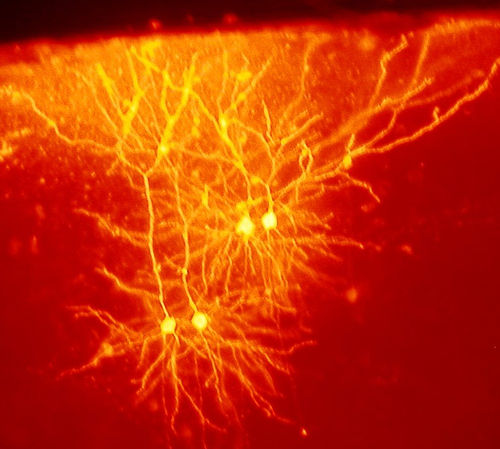
\includegraphics[width = 5cm]{./images/neurons.jpg}
  \hspace*{0.6cm}
  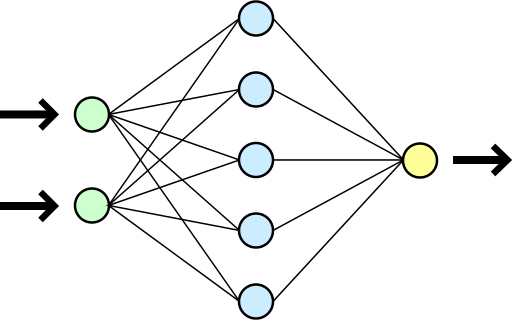
\includegraphics[width = 5cm]{./images/ANN.png}
  \footnote{\url{http://commons.wikimedia.org/wiki/File:Mouse_cingulate_cortex_neurons.jpg} \\ \url{http://commons.wikimedia.org/wiki/File:Neural_network.svg}}
\end{frame}

\note{
Artificial neural networks are used in classification and regression. The are inspired by the brain, which consists of a network of brain cells (neurons). Mathematically artifical neural networkds are a concatenation of weighted functions. An exemplary application is image processing. }


\begin{frame}{Support Vector Machines}
  \begin{center}
    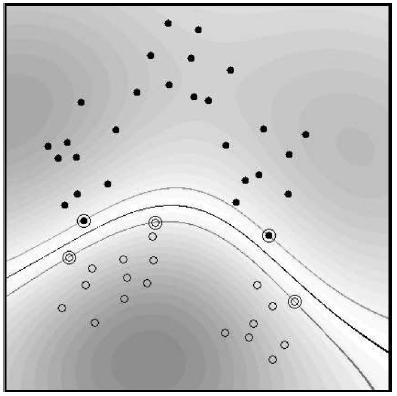
\includegraphics[width = 7cm]{./images/SVM.JPG}
    \footnote{\url{http://commons.wikimedia.org/wiki/File:Svm_10_perceptron.JPG}}
  \end{center}
\end{frame}

\note{
Support Vector Machines (SVM) were originally a classification method (regression is also possible). SVMs try to draw a border between to classes in the covariate space. The distance between the border and the class points is maximized. They use a mathematical trick to implicitly project the covariates in a space with higher dimensions (sounds a bit crazy but it is true) in order to achieve class separation. Text classification is an exemplary usage. 
}

\begin{frame}{Random Forests}
  \begin{center}
    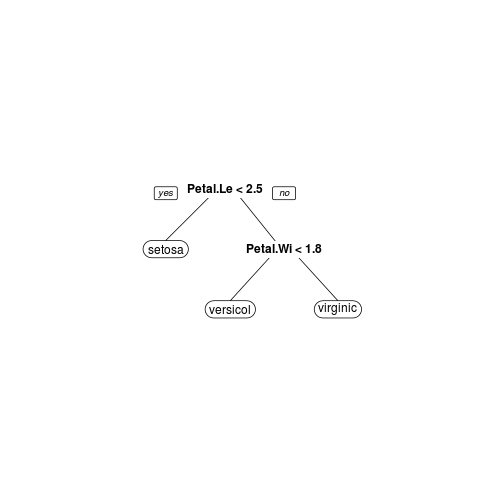
\includegraphics[width = 10cm, clip, trim = 3cm 0cm 3cm 4cm]{./images/tree.png}
  \end{center}
\end{frame}

\begin{frame}{Random Forests}
  \begin{center}
    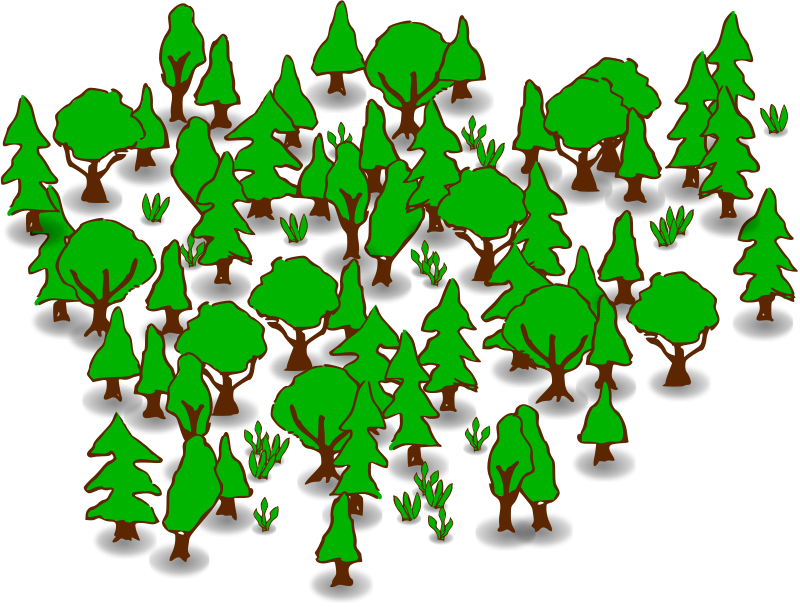
\includegraphics[width = 10cm]{./images/forest.png}
    \footnote{\url{http://openclipart.org/detail/175304/forest-by-z-175304}}
  \end{center}
\end{frame}

\note{
  Random Forests\texttrademark (invented by Leo Breiman) are used for regression und classifikation. A Random Forest consists of many decision trees. Two random mechanisms are used to train different trees on the data. Results from all trees are averaged for the prediction.
}

\section{Principles}
\captionslide{Statistical learning principles}

\begin{frame}{Rashomon Effect}
  \begin{center}
   (Often) Many different models describe a situation equally accurate. 
  \end{center}
\end{frame}

\note{
  Rashomon is a japanese movie in which four witnessess tell different versions about an observed crime. All versions account for the facts but they are contradictory. In terms of statistical learning this means, that often different models (e.g. same y but different covariates) can be equally accurate. Each model has a different interpretation which makes it difficult to find the true mechanism in the data modeling cultures. In the algorithmic modeling culture the Rashomon effect is exploited by aggregating over many models. Random forest use this effect when aggregating over many trees. It is also common to average the predictions from different algorithms. }

\begin{frame}{Dimensionality of the data}
  \begin{itemize}
  \item The higher the dimensionality of the data (\# covariates) the more difficult is the separation of signal and noise
  \item Common practice in data modeling: variable selection (by expert selection or data driven) and reduction of dimensionality (e.g. PCA)
  \item Common practice in algorithmic modeling: Engineering of new features (covariates) to increase predictive accuracy; algorithms robust for many covariates
  \end{itemize}
\end{frame}


\begin{frame}{Prediction vs. Interpretation}
  \begin{tikzpicture}
    \draw (0,0) -- (0,1.5) -- (9.9,0) -- (0,0);
    \draw  (0, 1.6) -- (10,1.6) -- (10, 0.1) -- (0, 1.6);
    \node at (3, 0.2) {Interpretability};
    \node at (7, 1.3) {Predictive accuracy};
    \node at (1.3, -0.5) {Tree};
    \node at (9, -0.5) {Random Forest};
    \node at (1.5, -1.2) {Logist. Regression};
    \node at (9, -1.2) {Neuronales Netz};
    \node at (1.3, -1.9) {\ldots};
    \node at (9, -1.9) {\ldots};
  \end{tikzpicture}
\end{frame}

\note{
There is a tradeoff between interpretability and predictive accuracy: the models that are good in prediction are often complex and models that are easy to interpret are often bad predictors. 
See for example trees and Random Forests: 
A single decision tree is very intuitive and easy to read for non-professionals, but they are instable and give weak predictions. A complex aggregation of decision trees (Random Forest) has an excellent prediction accuracy, but it is impossible to interpret the model structure. }

\begin{frame}{Goodness of model}
  \begin{itemize}
  \item Data modeling culture: Goodness of fit often base on model assumptions (e.g. AIC) and calculated on training data. 
  \item Algorithmic modeling culture: Evaluation of predictive accuracy with an extra test set or cross validation. 
  \end{itemize}
How good is a statistical model if the predictive accuracy is weak? Ist it legit to interpretate parameters and p-values?
\end{frame}


\section{Experiences}
\captionslide{Personal Experiences}

\begin{frame}[fragile]\frametitle{Statistical Consulting}
  Stereotypical user ...
  \begin{itemize}
  \item are e.g. veterinarians, linguists, biologists, \ldots
  \item crave p-values
  \item want interpretability
  \item ignore model diagnosis 
  \end{itemize}
\end{frame}

\note{
From my experience in the statistical consulting unit of our university, most user want to test their scientific hypthesis with models. They want models which are easy to interpret regarding their questions. Thus it is more important to have a model that gives parameters associated to covariates and p-values than to have a model that predicts the data well. 
}

\begin{frame}[fragile]\frametitle{kaggle}
  Algorithms of winners on kaggle,  a plattform für prediction challenges:
  \begin{itemize}
    % http://blog.kaggle.com/2013/05/06/qa-with-job-salary-prediction-first-prize-winner-vlad-mnih/
  \item  Job Salary Prediction: \doublequoted{I used deep neural networks}
    % http://blog.kaggle.com/2012/12/19/1st-place-observing-dark-worlds/
  \item Observing Dark Worlds: \doublequoted{Bayesian analysis provided the winning recipe for solving this problem}
    % http://blog.kaggle.com/2012/01/03/the-perfect-storm-meet-the-winners-of-give-me-some-credit/
  \item Give Me Some Credit: \doublequoted{In the end we only used five supervised learning methods: a random forest of classification trees, a random forest of regression trees, a classification tree boosting algorithm, a regression tree boosting algorithm, and a neural network.}
  \end{itemize}
\end{frame}

\note{
  Kaggle (\url{http://www.kaggle.com}) is a platform for prediction challenges. Data are provided and the participant with the best prediction on a test set wins the challenge. To generate insights about the mechanisms in the data is secondary because the prediction is all that counts to win. That's why the algorithmic modeling culture is superior in this field. 
}

\section{Fazit}
\begin{frame}{Conclusion}
  A data analysts should:
  \begin{itemize}
  \item Use predictive accuracy to evaluate models
  \item Seek the best model
  \item Add Machine Learning to their toolbox
  \end{itemize}
\end{frame}


\begin{frame}{Further literature}

\begin{thebibliography}{10} 
  \beamertemplatearticlebibitems
  \bibitem{breiman}
    L.~Breiman
    \newblock {\em Statistical modeling: The two cultures (with comments and a rejoinder by the author)}
    \newblock Institute of Mathematical Statistics, 2001.   
  \beamertemplatebookbibitems
  \bibitem{elements}
    T.~Hastie, R.~Tibshirani and J.~Friedman
    \newblock {\em The elements of statistical learning}
    \newblock Springer New York, 2001
  \end{thebibliography}
\end{frame}


\begin{frame}[plain]
  \addtocounter{framenumber}{-1}
 \doublequoted{All models are wrong, but some are useful} (G. Box)
\end{frame}


%% \begin{frame}{Other view}
%%   \begin{figure}
%%     \centering
%%     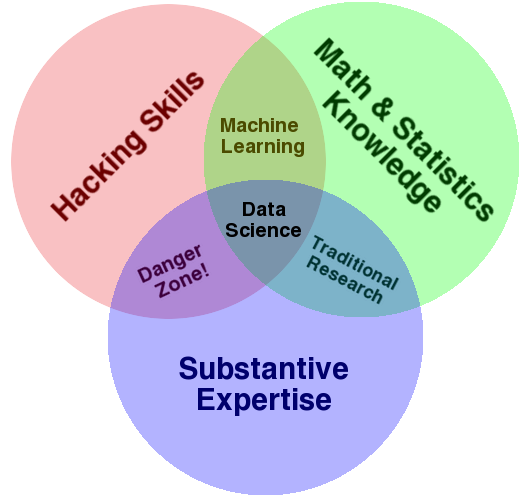
\includegraphics[width = 6cm]{./images/Data_Science_VD.png}
%%     \caption{\url{https://s3.amazonaws.com/aws.drewconway.com/viz/venn_diagram/data_science.html}}
%%   \end{figure}
%% \end{frame}

%% \note{
%%   Pragmatischere Sicht: \\
%%   Machine Learning ist die Schnittstelle zwischen Computer Science und Statistik.
%% }

\begin{frame}[plain]
  \addtocounter{framenumber}{-1}
  D.R. Cox in der Antwort auf Breiman's Paper: \\
  \vspace{0.5cm}
  \doublequoted{
    Descriptively appealing and transparent methods with a firm model base are the ideal.
  }
\end{frame}


\begin{frame}[plain]
  \addtocounter{framenumber}{-1}
  B. Efron in der Antwort auf Breiman's Paper: \\
\vspace{0.5cm}
  \doublequoted{
    we are being asked to face problems that never heard of good experimental design
  } \\
  Allerdings hält aber den Wert der Vorhersagegüte für überbewertet von Breiman. 

\end{frame}
\end{document}


